\section{Experimental results}
\label{sec:experiments}

We conducted our experiments using Amazon Mechanical
Turk~\footnote{http://www.mturk.com}, which allows workers (our pool
of prospective subjects) to perform small jobs for a fee through a Web
interface.  No specialized training or knowledge is typically expected
of the workers.  Amazon Mechanical Turk has been successfully used in
the past to develop gold-standard data for natural language
processing~\cite{snow-08} and to label images~\cite{imagenet-cvpr09}.

We prepare two randomly-chosen, 100-document subsets of English
Wikipedia~\footnote{http://en.wikipedia.org}.  For convenience, we
denote these two sets of documents as \emph{set1} and \emph{set2}.
For each document, we keep only the first 150 words for our
experiments.  Because of the encyclopedic nature of the corpus, the
first 150 words typically provides a broad overview of the themes in
the article.  We also removed from the corpus stop words and words
which occur infrequently\footnote{Infrequently occurring words were
  identified as those appearing fewer than eight times on a larger
  collection of 7726 articles.}, leading to a lexicon of 8263 words.
After this pruning \emph{set1} contained 11614 words and \emph{set2}
contained 11318 words.

Workers were asked to perform twenty of the taggings described in
\mysec{sec:tasks} for each task; workers were paid \$0.25 for each
such task.  The number of latent topics, $K$, is a free parameter.
Here we explore two values of this parameter, $K=10$ and $K=15$,
leading to a total of four experiments --- two for each set of
documents and two for each value of $K$.

\subsection{Tagging behavior}
For each experiment we issued 100 HITs, leading to a total of 2000
tags per experiment.  \myfig{fig:hists} shows the number of HITs
performed per person in each experiment.  Between 12 and 30 distinct
workers participated in each experiment.  The number of HITs performed
per person is heavily skewed, with the most active participants
completing an order of magnitude more HITs than other particpants.

\begin{figure*}
\centering
\subfigure[\emph{set1}, $K = 10$]{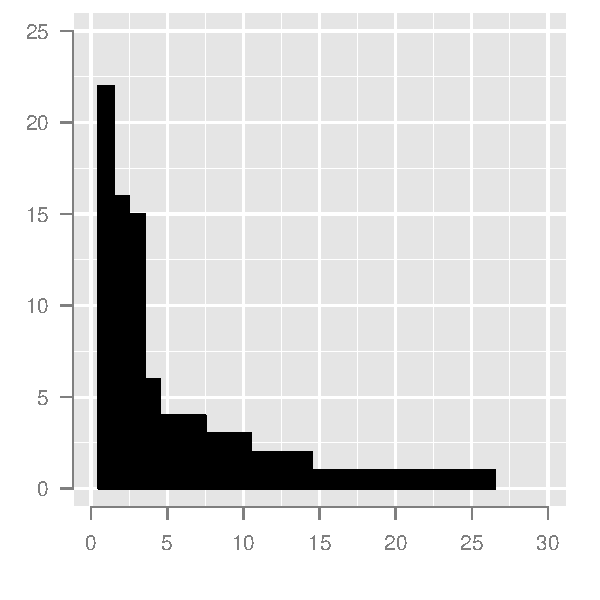
\includegraphics[width = .24\linewidth]{figures/histogram_1}}%
\subfigure[\emph{set1}, $K = 15$]{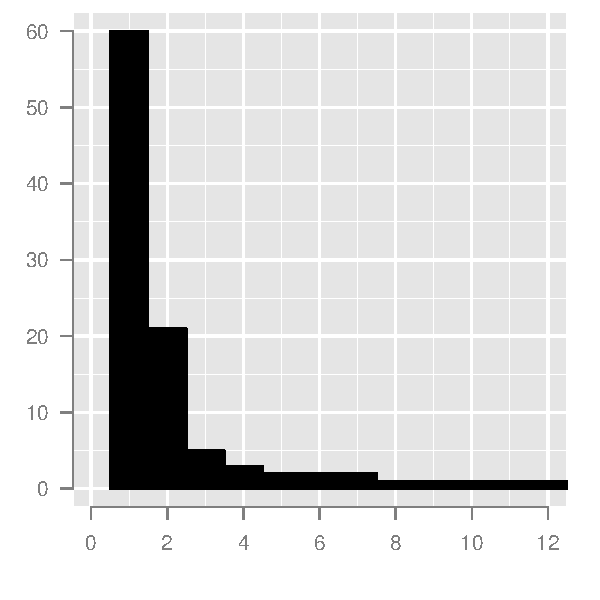
\includegraphics[width = .24\linewidth]{figures/histogram_2}}%
\subfigure[\emph{set2}, $K = 10$]{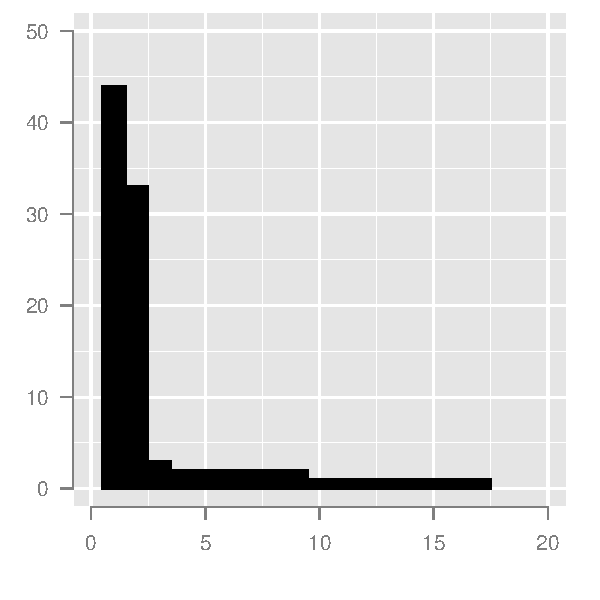
\includegraphics[width = .24\linewidth]{figures/histogram_4}}%
\subfigure[\emph{set2}, $K = 15$]{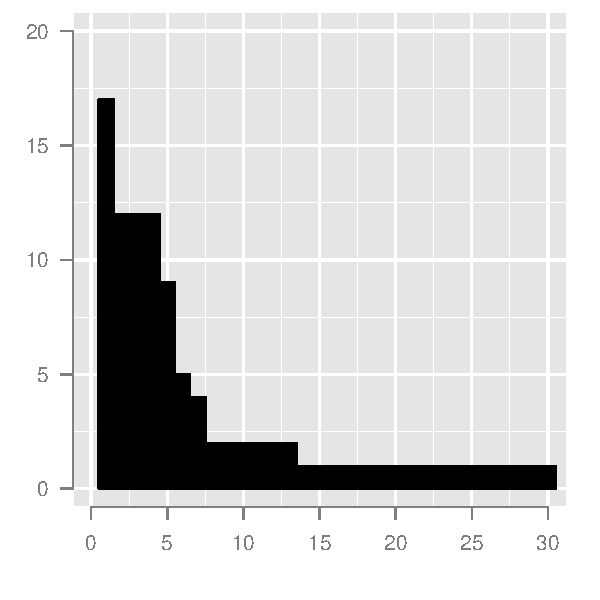
\includegraphics[width = .24\linewidth]{figures/histogram_3}}%
\caption{The number of HITs performed by participant. Between 12 and 30 people participated in each experiment.}
\label{fig:hists}
\end{figure*}

\begin{figure}
\centering
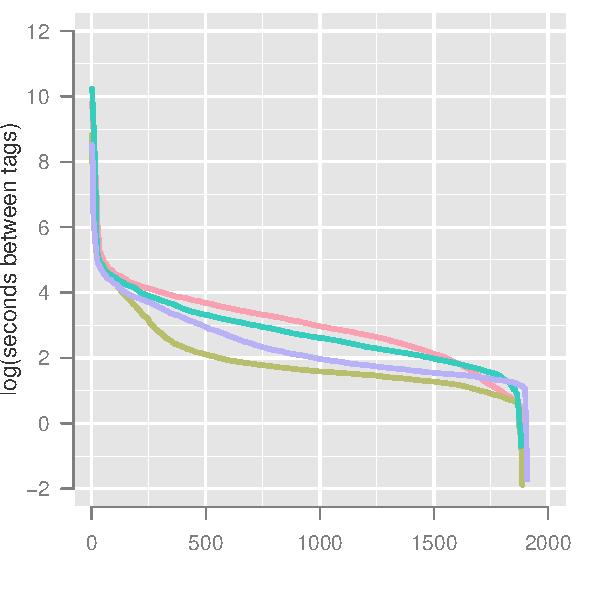
\includegraphics[width = .9\linewidth]{figures/hit_times}
\caption{The distribution of times taken per HIT.  Each series represents a different experiment.  The bulk of the tags took less than one minute and more than a few seconds.}
\label{fig:times}
\end{figure}

\myfig{fig:times} shows the amount of time taken per tag, in log
seconds. Each color represents a different experiment.  The bulk of
the tags took less than a minute to perform and more than a few
seconds.

\begin{table*}
  \caption{The five words with the highest probability mass in each topic inferred by humans using the task described in \mysec{sec:tasks}.  Each subtable shows the results for a particular experimental setup.   Each row is a topic; the most probable words are ordered from left to right.}
\label{tab:topic-samples}
\centering
\footnotesize
\hspace*{-.4in}
\subfigure[\emph{set1}, $K = 10$]{
\begin{tabular}{lllll}
  railway & lighthouse & rail & huddersfield & station \\ \hline 
  school & college & education & history & conference \\ \hline 
  catholic & church & film & music & actor \\ \hline 
  runners & team & championships & match & racing \\ \hline 
  engine & company & power & dwight & engines \\ \hline 
  university & london & british & college & county \\ \hline 
  food & novel & book & series & superman \\ \hline 
  november & february & april & august & december \\ \hline 
  paint & photographs & american & austin & black \\ \hline 
   war & history & army & american & battle \\ 
\end{tabular}
}%
\subfigure[\emph{set2}, $K = 10$]{
  \begin{tabular}{|lllll}
    president & emperor & politician & election & government \\ \hline 
    american & players & swedish & team & zealand \\ \hline 
    war & world & navy & road & torpedo \\ \hline 
    system & pop & microsoft & music & singer \\ \hline 
    september & 2007 & october & december & 1999 \\ \hline 
    television & dog & name & george & film \\ \hline 
    people & malay & town & tribes & cliff \\ \hline 
    diet & chest & enzyme & hair & therapy \\ \hline 
    british & city & london & english & county \\ \hline 
    school & university & college & church & center \\
  \end{tabular}
}
\hspace*{-.5in}
\subfigure[\emph{set1}, $K = 15$]{
\begin{tabular}{lllll}
australia & knee & british & israel & set \\ \hline 
  catholic & roman & island & village & columbia \\ \hline 
  john & devon & michael & austin & charles \\ \hline 
  school & university & class & community & district \\ \hline 
  november & february & 2007 & 2009 & 2005 \\ \hline 
  lighthouse & period & architects & construction & design \\ \hline 
  railway & rail & huddersfield & ownership & services \\ \hline 
  cyprus & archdiocese & diocese & king & miss \\ \hline 
  carson & gordon & hugo & ward & whitney \\ \hline 
  significant & application & campaign & comic & considered \\ \hline 
  born & london & american & england & black \\ \hline 
  war & defense & history & military & artillery \\ \hline 
  actor & film & actress & band & designer \\ \hline 
  york & michigan & florida & north & photographs \\ \hline 
  church & catholic & county & 2001 & agricultural \\ 
\end{tabular}
}%
\subfigure[\emph{set2}, $K = 15$]{
\begin{tabular}{|lllll}
  music & pop & records & singer & artist \\ \hline 
  film & paintings & movie & painting & art \\ \hline 
  school & university & english & students & british \\ \hline 
  drama & headquarters & chess & poet & stories \\ \hline 
  family & church & sea & christmas & emperor \\ \hline 
  dog & broadcast & television & bbc & breed \\ \hline 
  champagne & regular & character & characteristic & common \\ \hline 
  election & government & parliament & minister & politician \\ \hline 
  enzyme & diet & protein & hair & oxygen \\ \hline 
  war & navy & weapons & aircraft & military \\ \hline 
  september & october & december & 2008 & 1967 \\ \hline 
  district & town & marin & america & american \\ \hline 
  car & power & system & device & devices \\ \hline 
  hockey & players & football & therapy & champions \\ \hline 
  california & zealand & georgia & india & kolkata \\
\end{tabular}
}
\vspace{0.2in}
\end{table*}

\begin{figure*}
\centering
\subfigure[$K = 10$]{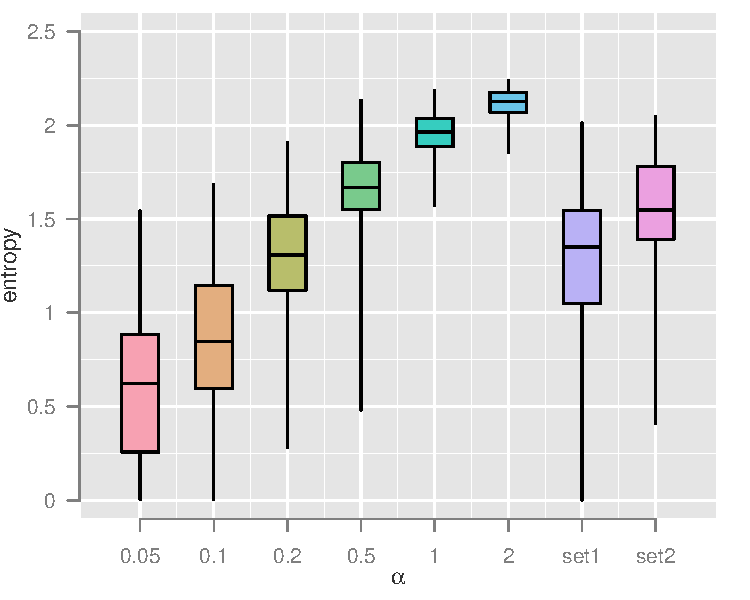
\includegraphics[width = .42\linewidth]{figures/entropy_K10}}%
\subfigure[$K = 15$]{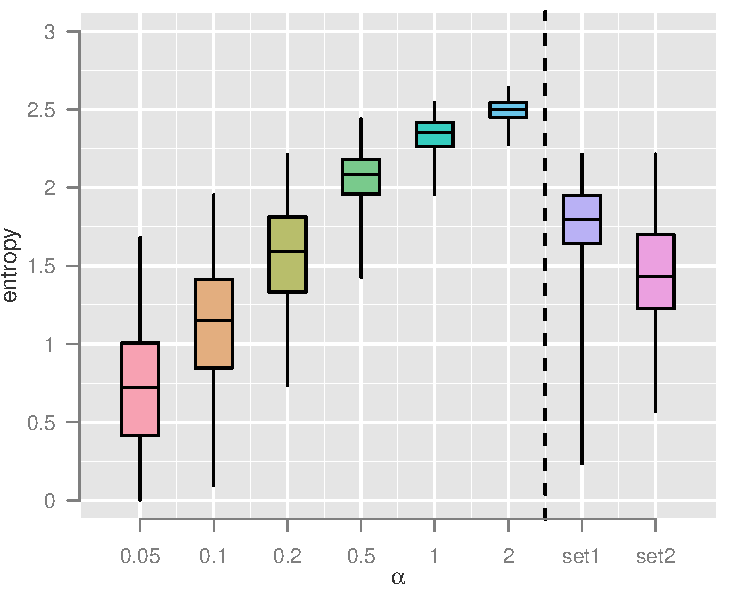
\includegraphics[width = .42\linewidth]{figures/entropy_K15}}

\caption{A comparison of the entropy of distributions drawn from a
  Dirichlet versus the entropy of the topic proportions inferred by
  workers.  Each column of the boxplot shows the distribution of
  entropies for 100 draws from a Dirichlet distribution with parameter
  $\alpha$.  The two rightmost columns show the distribution of the
  entropy of the topic proportions inferred by workers on \emph{set1}
  and \emph{set2}.  The $\alpha$ workers typically falls between 0.2
  and 0.5.}

\label{fig:entropy}
\end{figure*}

\subsection{Comparison with LDA}
\begin{figure*}
\centering
%\subfigure[\emph{full}, $K = 10$]{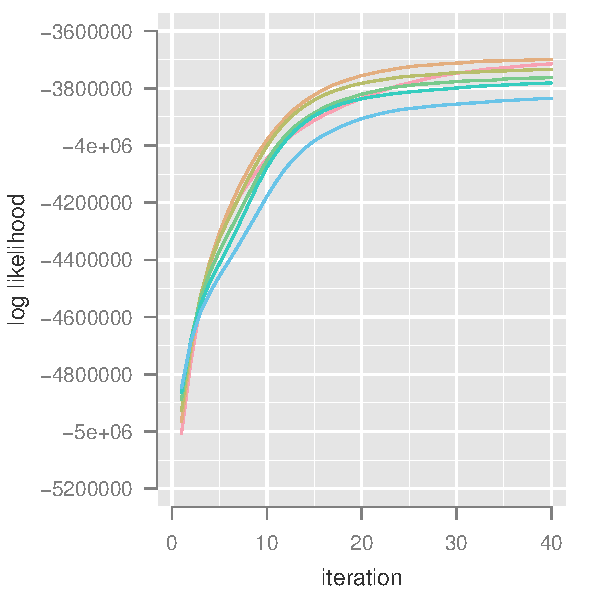
\includegraphics[width = .32\linewidth]{figures/lda_ll_full_10}}%
\subfigure[\emph{set1}, $K = 10$]{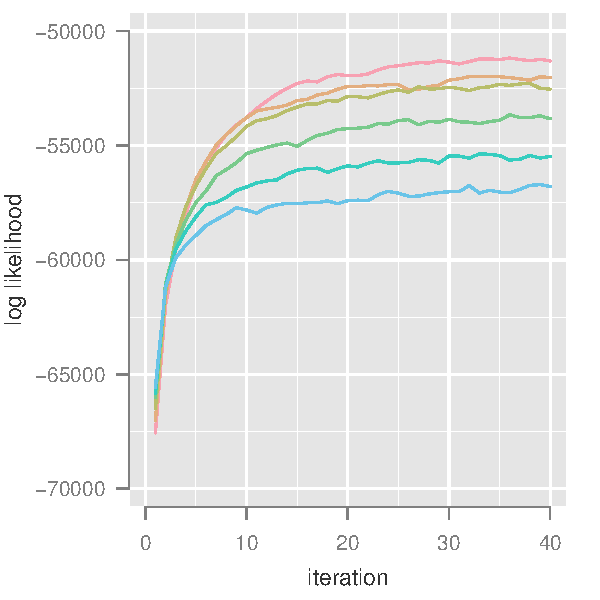
\includegraphics[width = .24\linewidth]{figures/lda_ll_set1_10}}%
\subfigure[\emph{set2}, $K = 10$]{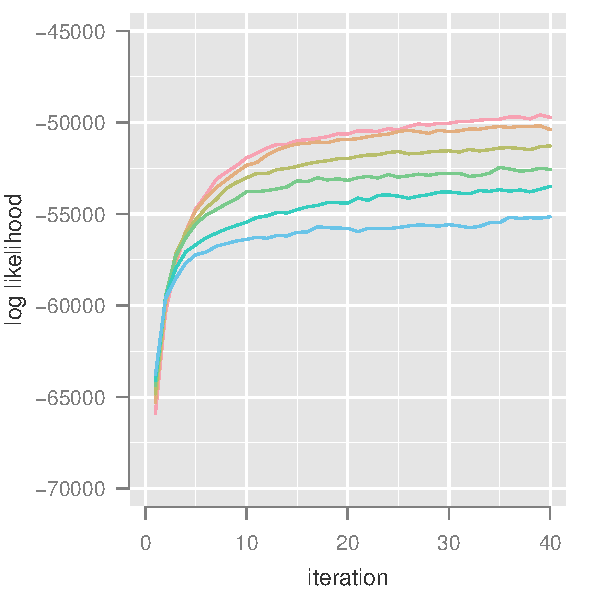
\includegraphics[width = .24\linewidth]{figures/lda_ll_set2_10}}%
%\subfigure[\emph{full}, $K = 15$]{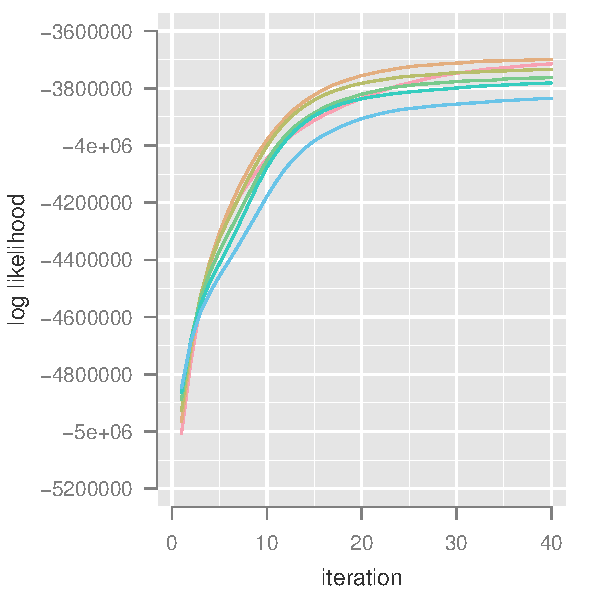
\includegraphics[width = .32\linewidth]{figures/lda_ll_full_10}}%
\subfigure[\emph{set1}, $K = 15$]{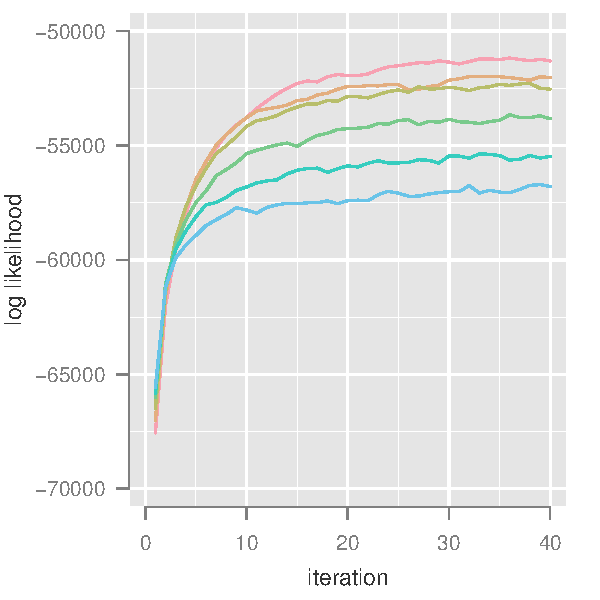
\includegraphics[width = .24\linewidth]{figures/lda_ll_set1_10}}%
\subfigure[\emph{set2}, $K = 15$]{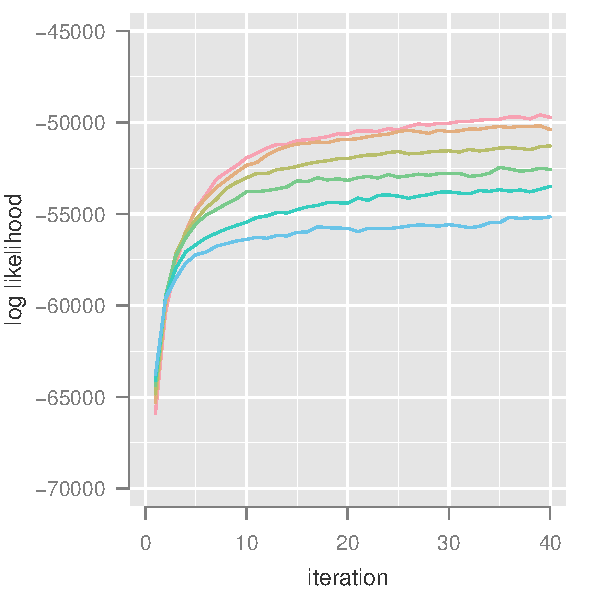
\includegraphics[width = .24\linewidth]{figures/lda_ll_set2_10}}

\caption{The log-likelihood achieved by LDA as a function of iteration.  
%\emph{full} refers to a larger set of 7726 Wikipedia articles.   
There is one series for each value of $\alpha \in \{0.05, 0.1, 0.2, 0.5, 1.0, 2.0\}$ from top to bottom.}
\label{fig:ll}
\end{figure*}

\begin{table*}[ht]
\footnotesize
\centering
  \caption{The five words with the highest probability mass in each topic inferred by LDA, with $\alpha = 0.2$.  Each subtable shows the results for a particular experimental setup.   Each row is a topic; the most probable words are ordered from left to right.}
\label{tab:lda-topic-samples}
\hspace*{-.1in}
\subfigure[\emph{set1}, $K=10$]{
\begin{tabular}{lllll}
born & 2004 & team & award & sydney \\ \hline 
  regiment & army & artillery & served & scouting \\ \hline 
  line & station & main & island & railway \\ \hline 
  region & street & located & site & knee \\ \hline 
  food & february & conference & day & 2009 \\ \hline 
  pride & greek & knowledge & portland & study \\ \hline 
  catholic & church & roman & black & time \\ \hline 
  class & series & film & actor & engine \\ \hline 
  travel & human & office & management & defense \\ \hline 
  school & born & war & world & university \\ 
\end{tabular}
}%
\subfigure[\emph{set2}, $K=10$]{
\begin{tabular}{|lllll}
september & english & edit & nord & hockey \\ \hline 
  black & hole & current & england & model \\ \hline 
  training & program & war & election & navy \\ \hline 
  school & university & district & city & college \\ \hline 
  family & word & international & road & japan \\ \hline 
  publication & time & day & india & bridge \\ \hline 
  born & pop & world & released & march \\ \hline 
  won & video & microsoft & project & hungary \\ \hline 
  film & hair & bank & national & town \\ \hline 
  people & name & french & therapy & artist \\ 
\end{tabular}
}
\hspace*{-.3in}
\subfigure[\emph{set1}, $K=15$]{
\begin{tabular}{lllll}
time & michael & written & experience & match \\ \hline 
  line & station & railway & branch & knowledge \\ \hline 
  film & land & pass & set & battle \\ \hline 
  william & florida & carson & virginia & newfoundland \\ \hline 
  war & regiment & british & army & south \\ \hline 
  reaction & terminal & copper & running & complex \\ \hline 
  born & school & world & college & black \\ \hline 
  food & conference & flight & medium & rail \\ \hline 
  township & scouting & census & square & county \\ \hline 
  travel & defense & training & management & edges \\ \hline 
  series & actor & engine & november & award \\ \hline 
  pride & portland & band & northwest & god \\ \hline 
  team & knee & 2004 & sydney & israel \\ \hline 
  catholic & located & site & region & church \\ \hline 
  class & february & time & public & king \\ 
\end{tabular}
}%
\subfigure[\emph{set2}, $K=15$]{
\begin{tabular}{|lllll}
family & protein & enzyme & acting & oxygen \\ \hline 
  england & producer & popular & canadian & sea \\ \hline 
  system & death & artist & running & car \\ \hline 
  character & series & dark & main & village \\ \hline 
  english & word & publication & stream & day \\ \hline 
  training & program & hair & students & electrical \\ \hline 
  district & town & city & local & kolkata \\ \hline 
  september & edit & music & records & recorded \\ \hline 
  black & pop & bank & usually & hole \\ \hline 
  people & choir & road & diet & related \\ \hline 
  war & built & navy & british & service \\ \hline 
  center & million & cut & champagne & players \\ \hline 
  born & television & current & drama & won \\ \hline 
  school & university & college & election & born \\ \hline 
  film & nord & played & league & hockey \\ 
\end{tabular}
}
\end{table*}

\paragraph{Learned topics} As described in \mysec{sec:tasks}, the tag-and-cluster
task is a way of allowing humans to construct a topic model.  One way
of visualizing a learned topic model is by examining its topics.
\mytab{tab:topic-samples} shows the topics constructed by human
judgments.  Each subtable shows a different experimental setup and
each row shows an individual topic.  The five most frequently
occurring words in each topic are shown, ordered from left to right.

Many of the topics inferred by humans have straightforward
interpretations.  For example, the \{\texttt{november, february,
  april, august, december}\} topic for the \emph{set1} corpus with
$K=10$ is simply a collection of months.  Similar topics (with years
and months combined) can be found in the other experimental
configurations.  Other topics also cover specific semantic domains,
such as \{\texttt{president, emperor, politican, election,
  government}\} or \{\texttt{music, pop, records, singer, artist}\}.
Several of the topics are combinations of distinct concepts, such as
\{\texttt{catholic, church, film, music, actor}\}, which is often
indicative of the number of clusters, $K$, being too low.

\mytab{tab:lda-topic-samples} shows the topics learned by LDA under
the same experimental conditions, with the Dirichlet hyperparameter
$\alpha = 0.2$.  These topics are more difficult to interpret than the
ones created by humans.  Some topics seem to largely make sense except
for some anomalous words, such as \{\texttt{district, town, city,
  local, kolkata}\} or \{\texttt{school, university, college,
  election, born}\}.  But the small amount of data means that it is
difficult for a model which does not leverage prior knowledge to infer
meaningful topic.  In contrast, several humans, even working
independently, can leverage prior knowledge to construct meaningful
topics with little data.

There is another qualitative difference between the topics found by
the tag-and-cluster task and LDA.  Whereas LDA must rely on
co-occurrence, humans can use ontological information.  Thus, a topic
which has ontological meaning, such as a list of months, may rarely be
discovered by LDA since the co-occurrence patterns of months do not
form a strong pattern.  But users in every experimental configuration
constructed this topic, suggesting that the users were consistently
leveraging information that would not be available to LDA, even with a
larger corpus.

\paragraph{Hyperparameter values} A persistent question among
practitioners of topic models is how to set or learn the value of the
hyperparameter $\alpha$.  $\alpha$ is a Dirichlet parameter which acts
a control on sparsity --- smaller values of $\alpha$ lead to sparser
document-topic distributions.  By comparing the sparsity patterns of
human judgments to those of LDA for different settings of $\alpha$, we
can infer the value of $\alpha$ that would best match human judgments.

\myfig{fig:entropy} shows a boxplot comparison of the entropy of draws
from a Dirichlet distribution (the generative process in LDA), versus
the observed entropy of the models learned by humans.  The first six
columns show the distributions for the Dirichlet draws for various
values of $\alpha$; the last two columns show the observed entropy
distributions on the two corpora, \emph{set1} and \emph{set2}.

The empirical entropy distributions across the corpora are comparable
to those of a Dirichlet distribution with $\alpha$ between
approximately $0.2$ and $0.5$.  These settings of $\alpha$ are
slightly higher than, but still in line with a common rule-of-thumb of
$\alpha = 1 / K$.  \myfig{fig:ll} shows the log-likelihood, a measure
of model fit, achieved by LDA for each value of $\alpha$.  Higher
log-likelihoods indicate better fits.  Commensurate with the rule of
thumb, using log-likelihoods to select $\alpha$ would encourage values
smaller than human judgments.

However, while the entropy of the Dirichlet draws increases
significantly when the number of clusters is increased from $K=10$ to
$K=15$, the entropies assigned by humans does not vary as
dramatically.  This suggests that for any given document, humans are
likely to pull words from only a small number of topics, regardless of
how many topics are available, whereas a model will continue to spread
probability mass across all topics even as the number of topics
increases.
